\chapter{TD strain tensor with surface relaxation}
\label{Chap:strainMatrix}

Semi-infinite threading dislocation normal to a surface strain tensor, $\epsilon_{ij}$,  shown as contour plots for each component. 

\begin{equation*}
    \epsilon_{ij} = \begin{pmatrix}
    \epsilon_{11} & \epsilon_{12} & \epsilon_{13} \\
    \epsilon_{21} & \epsilon_{22} & \epsilon_{23} \\
    \epsilon_{31} & \epsilon_{32} & \epsilon_{33} \\
    \end{pmatrix}.
\end{equation*}

Where the elastic strain has the following property : $\epsilon_{ij}=\epsilon_{ji}$ making these matrices symmetric with respect to their diagonal. Fig.~\ref{Fig:screwMatrix} shows the strain components as contour plots for a screw threading dislocation and   Fig.~\ref{Fig:edgeMatrix} for an edge TD.
%---------
\begin{sidewaysfigure}[ht]
    \centering
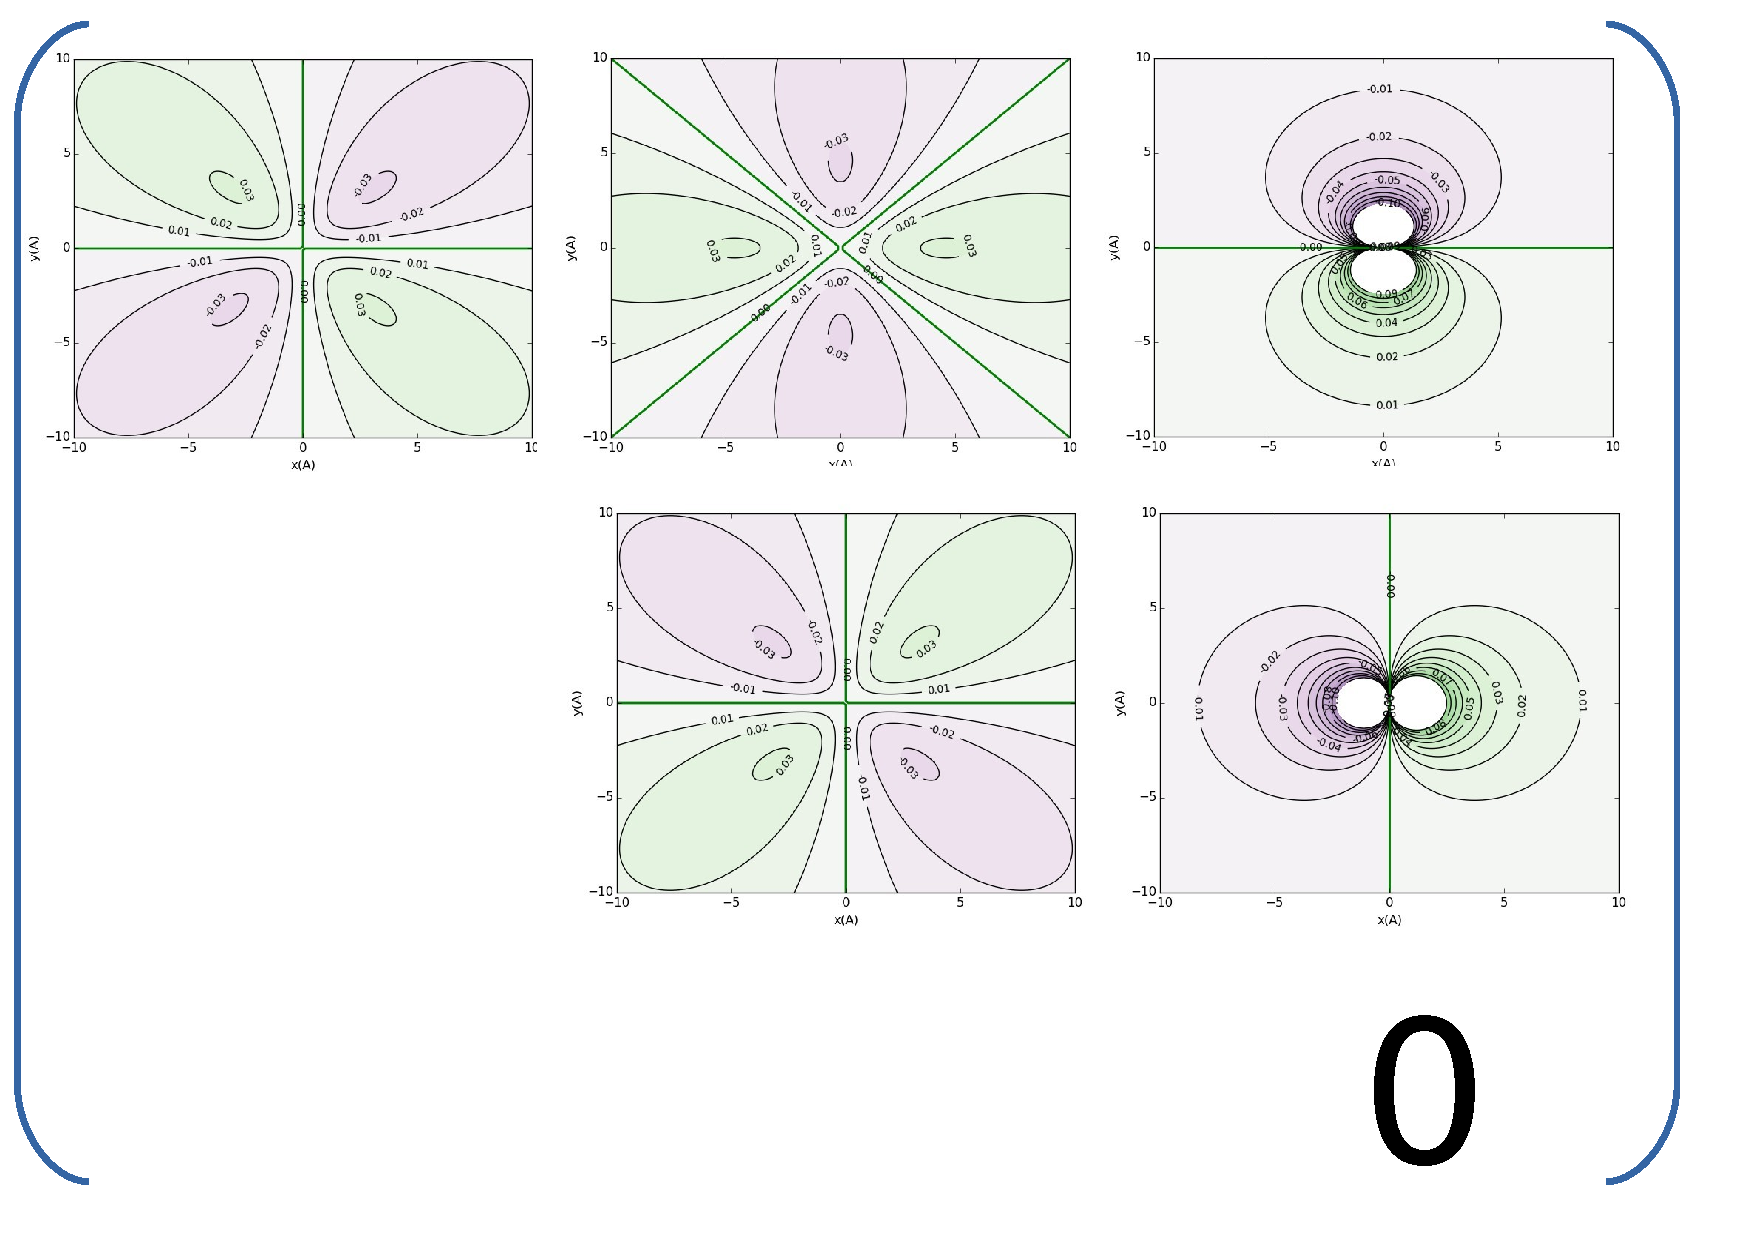
\includegraphics[width=1\linewidth]{Figures/screw_matrix.pdf}
\caption[Screw TD strain tensor.]{Strain field tensor components of a screw TD in GaN normal to a surface as contour plots. The strain is plotted on a $10 \times 10$ \si{\angstrom} plane centred on the dislocation and \SI{2}{\angstrom} below the surface.  }
\label{Fig:screwMatrix}
\end{sidewaysfigure}
%---------



%---------
\begin{sidewaysfigure}[ht]
    \centering
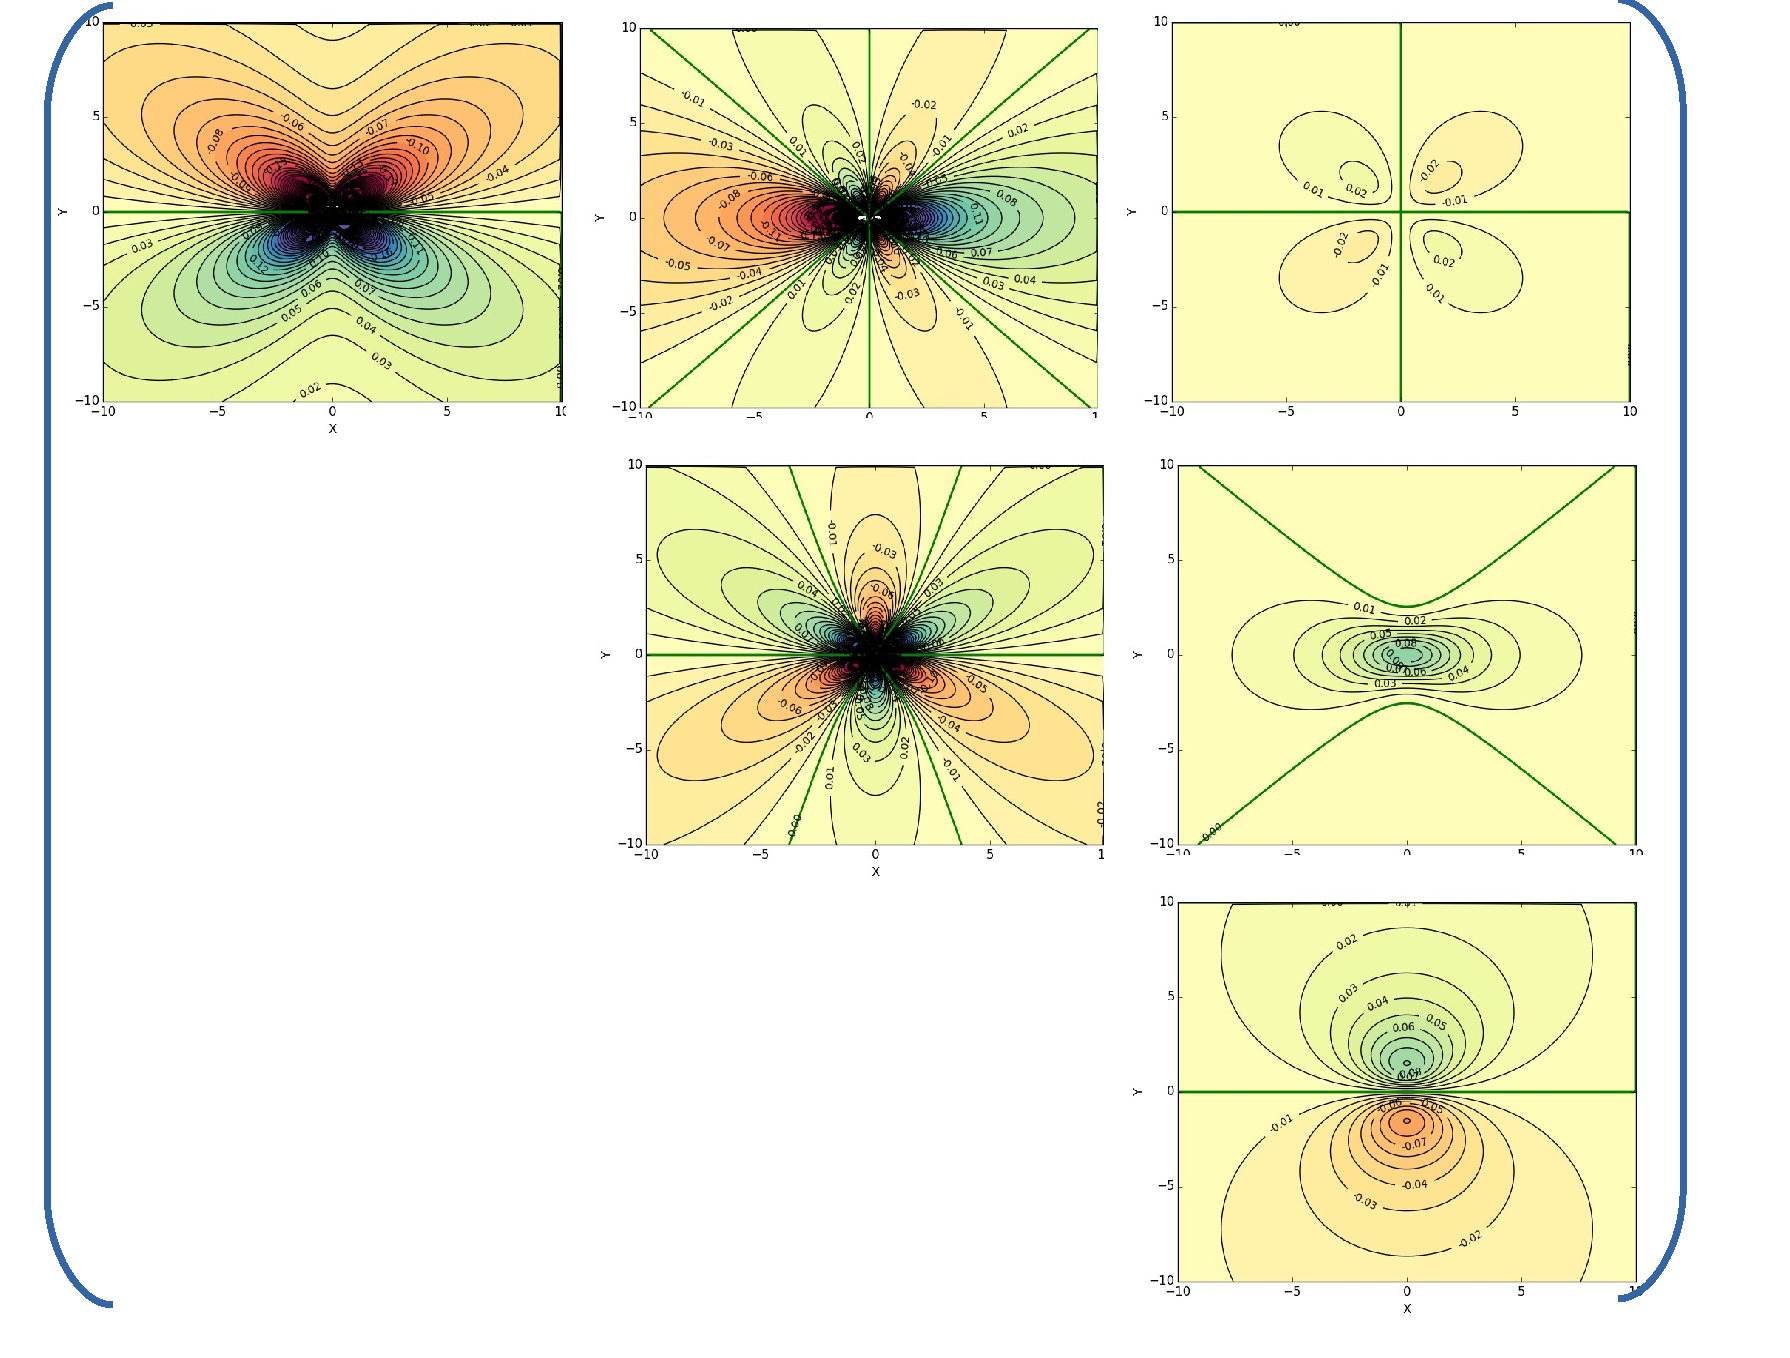
\includegraphics[width=1\linewidth]{Figures/edge_matrix.pdf}
\caption[Edge TD strain tensor.]{Strain field tensor components of an edge TD in GaN normal to a surface as contour plots. The strain is plotted on a $10 \times 10$ \si{\angstrom} plane centred on the dislocation and \SI{2}{\angstrom} below the surface.  }
\label{Fig:edgeMatrix}
\end{sidewaysfigure}
%---------

